
\documentclass{article}

% Extra colours; need to be first
\usepackage[usenames,dvipsnames,svgnames,table]{xcolor}

% Basic packages
\usepackage[utf8]{inputenc}
\usepackage[T1]{fontenc}

% URL
\usepackage{hyperref}

% Mono font
\usepackage[scaled]{beramono}

% Spacing
\usepackage{xspace}

% Table
\usepackage{booktabs}
\usepackage{tabularx}
\usepackage{multirow}

% Floating placement
\usepackage{placeins}
% use \FloatBarrier before a \section to ensure all floating are displayed
% before the new section

% Caption styling
\usepackage[justification=centering]{caption}

% Additional colours
\definecolor{c1}{HTML}{006C71}
\definecolor{c2}{HTML}{005155}
\definecolor{c3}{HTML}{FF8928}
\definecolor{c4}{HTML}{E86900}
\colorlet{ImportantCode}{ForestGreen}
\colorlet{ImportantCode2}{RubineRed}
\colorlet{ImportantCode3}{RedOrange}


% TIKZ
\usepackage{tikz}
\usetikzlibrary{shapes,fit,backgrounds,arrows,positioning,chains,patterns}

% for caching tikz pictures
\usetikzlibrary{external}
\tikzexternalize[prefix=tikz-figures/]
\pgfrealjobname{tikz}


% Listings
\usepackage{listings}
\usepackage{lstscala}
\lstloadlanguages{[ANSI]C}

\lstdefinelanguage{C99}[ANSI]{C}{
  basicstyle=\ttfamily,
  commentstyle=\color{lstscalacmt},
  morekeywords={bool,int32\_t},
  keywordstyle=\color{blue!30!darkgray}\bfseries,
  moredelim=**[is][\color{ImportantCode}]{@}{@},
  moredelim=**[is][\color{ImportantCode2}]{§}{§},
  moredelim=**[is][\color{ImportantCode3}]{£}{£},
}

\lstdefinelanguage{MyScala}{ % Using `Scala` result in a infinite recursion
  style=scala-color,
  morekeywords={[2]Unit,Boolean,Int},
  %keywordstyle={[2]\color{blue!30!darkgray}\bfseries}
}

\newcommand{\inlinecode}[1]{\lstinline[basicstyle=\ttfamily]|#1|}
\newcommand{\inlineC}[1]{\lstinline[language=C99]|#1|}
\newcommand{\inlineScala}[1]{\lstinline[language=MyScala]|#1|}
%\newcommand{\inlineScala}[1]{\lstinline[language=MyScala,breaklines=true,breakatwhitespace=true]|#1|}

%\lstset{aboveskip=5pt,belowskip=10pt}
\lstset{captionpos=b,abovecaptionskip=1em}

% For long listings
\lstdefinestyle{LongCode}{
  %aboveskip=1ex,
  basicstyle=\small\ttfamily,
  %belowskip=1ex,
  breaklines=true,
  postbreak=\raisebox{0ex}[0ex][0ex]{\ensuremath{\color{red}\hookrightarrow}},
  breakautoindent=false,
  %breakatwhitespace=false,
  %columns=fullflexible,
  framerule=0pt,
  framexrightmargin=0em,
  framexleftmargin=0em,
  numbers=left,
  numberstyle=\footnotesize\sffamily,
  tabsize=2
}



% Tables
\newcommand{\heading}[1]{\multicolumn{1}{c}{\textbf{#1}}}
\newcommand{\vheading}[1]{\rotatebox[origin=c]{90}{~\textbf{#1}~}}


% To centre table too wide
% credit: http://tex.stackexchange.com/a/27099/77356
\makeatletter
\newcommand*{\centerfloat}{%
  \parindent \z@
  \leftskip \z@ \@plus 1fil \@minus \textwidth
  \rightskip\leftskip
  \parfillskip \z@skip}
\makeatother



% General styling
%\newcommand{\sectionbreak}{\clearpage}



% Additional macros
\newcommand{\TODO}[1]{\texttt{\textcolor{YellowOrange}{(#1)}}} % for inline TODO
\newcommand{\GenC}{\emph{GenC}\xspace}





%%%

\title{From Verified Functions to Safe C Code}

\date{January 2016}

\author{Marco Antognini}

\begin{document}

\maketitle

\vfill

\begin{center}
    Optional Master Semester Project under the supervision of \\
    Viktor Kuncak \\
    Lab for Automated Reasoning and Analysis LARA - EPFL
\end{center}

\begin{center}
    
\includegraphics[width = 40mm]{res/epfl-logo}
\end{center}

\pagenumbering{gobble}
\newpage
\pagenumbering{arabic}


%\tableofcontents



\section{Overview}

As software becomes more and more complex we need ways to ensure it works
according to its specification. While hardware is more and more reliable and
cheaper, even for extreme environments such as space exploration (e.g.
spacecraft) or medical device (e.g. pacemaker), software development costs
substantially increase when programs have to be robust and safe. Many companies
spend a significant part of their budget in making sure their software won't put
people's life in danger or result in a huge monetary loss.

Leon\footnote{\url{http://leon.epfl.ch}} works at solving this issue for
programs written in (a subset of) Scala by providing tools to verify contracts,
repair erroneous implementations or even synthesis code. However, Scala being
based on JVM runtime, such tools are close to worthless for many companies that
run their software on very small devices: the lack of memory and CPU resources
prevents running virtualised code on such hardware. This explains why those
systems are written in low-level, C-like languages.

We therefore extend Leon to generate standard C99 code from a subset of Scala in
order to benefit from the high-level features of this language and reduce the
development cost of low-level software while avoiding using error-prone
languages.

\begin{figure}[h]
  \centering
  \beginpgfgraphicnamed{dev-pipeline}
  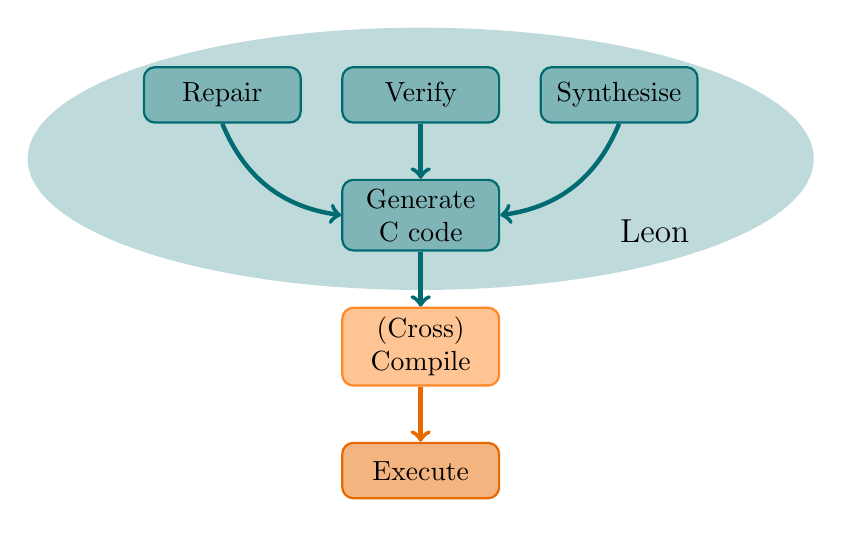
\begin{tikzpicture}
    [auto,
     box/.style   ={rectangle, draw=#1, thick, fill=#1!50,
                    text width=5em, text centered, rounded corners,
                    minimum height=2em},
     step/.style  ={circle, draw=#1, thick, fill=#1!50,
                    text width=2em, text centered,
                    minimum height=1em}
    ]

    \matrix [column sep=5mm,row sep=7mm]
    {
      % row 1
      \node [box=c1] (repair) {Repair}; &
      \node [box=c1] (verify) {Verify}; &
      \node [box=c1] (synthesise) {Synthesise}; \\
      % row 2
      & \node [box=c1] (genc) {Generate C code}; & \\
      % row 3
      & \node [box=c3] (compile) {(Cross) Compile}; & \\
      % row 4
      & \node [box=c4] (execute) {Execute}; & \\
    };

    \begin{scope}[every node/.style={font=\small\itshape}]
      \draw [ultra thick, ->, c1] (repair.south) to [bend right=30] (genc.west);
      \draw [ultra thick, ->, c1] (verify.south) to (genc.north);
      \draw [ultra thick, ->, c1] (synthesise.south) to [bend left=30] (genc.east);
      \draw [ultra thick, ->, c1] (genc.south) to (compile.north);
      \draw [ultra thick, ->, c4] (compile.south) to (execute.north);
    \end{scope}

    \begin{pgfonlayer}{background}
      \node[fill=c1!50,opacity=.5,inner sep=0pt,ellipse,
            fit=(repair) (verify) (synthesise) (genc)] (leon) {};
      \node[above left, font=\large] at (leon.south east) {Leon};
    \end{pgfonlayer}
  \end{tikzpicture}
  \endpgfgraphicnamed
  \caption{Development Process}
  \label{fig:dev-pipeline}
\end{figure}

The overall, high level development pipeline is illustrated in Figure
\ref{fig:dev-pipeline}. The first step is to generate a valid and verified Scala
program using Leon. The input source code should contains only one top-level
Scala \inlineScala{object} that represents the program to be converted. Then the
program can be converted into an equivalent C99 code through the \GenC phase
using the \inlinecode{\--genc} command line option.  Please refer to Leon's
manual for the complete invocation details as well as detailed explanation on
how to verify, repair or synthesis programs, and more.

The produced code can then be compiled using any standard-compliant C99 compiler
-- for example Clang\footnote{\url{http://clang.llvm.org/}} or
GCC\footnote{\url{https://gcc.gnu.org/}} -- to generate a native and optimised
assembly code for specific hardware architectures.  Then the compiled program
can be shipped to the desired hardware and executed as usual.



\section{Implementation Details}

In this section we give an overview of the generated C99 code and its structure,
plus some general insight on the implementation of \GenC inside Leon.



\subsection{Generated C99 Code}

The translated code follows a strict structure imposed by the difference between
the Scala and C languages. The main reason for this structure is that, in Scala,
the order of type and function definitions have little importance from a
compiler perspective but in C every type of function has to be at defined, or at
least declared, before being used. That is why the outputted code starts by
\inlineC{#include}'ing the necessary headers, then forward-declares every custom
data types -- such as tuples, case classes and arrays types presented in
Section~\ref{sec:types} -- so that their declarations, which follows next, can
refer to each other if needed. After data types, the same strategy is applied to
user-defined functions: first they are declared, in any order, and then their
bodies are fully defined.

A complete example of generated safe C code is presented in Appendix
\ref{sec:case-study-output-code}.



\subsection{GenC Phase in Leon}

The \GenC pipeline is made of several independent phases, that were already
defined in Leon, as shown in Figure~\ref{fig:genc-pipeline} where the
\inlineScala{PreprocessingPhase} is detailed in the right column with disabled
sub-phases represented by grey boxes. The roles of the three first phases are to
extract the Scala Abstract Syntax Tree (AST) from the input source code,
pre-process it to add Leon-specific information and transform it into a usable
format for the \inlineScala{GenerateCPhase}. This latter phase will produced a C
AST from its input so that the last phase can pretty print it into a given file.

\begin{figure}[h!]
  \centering
  \beginpgfgraphicnamed{genc-pipeline}
  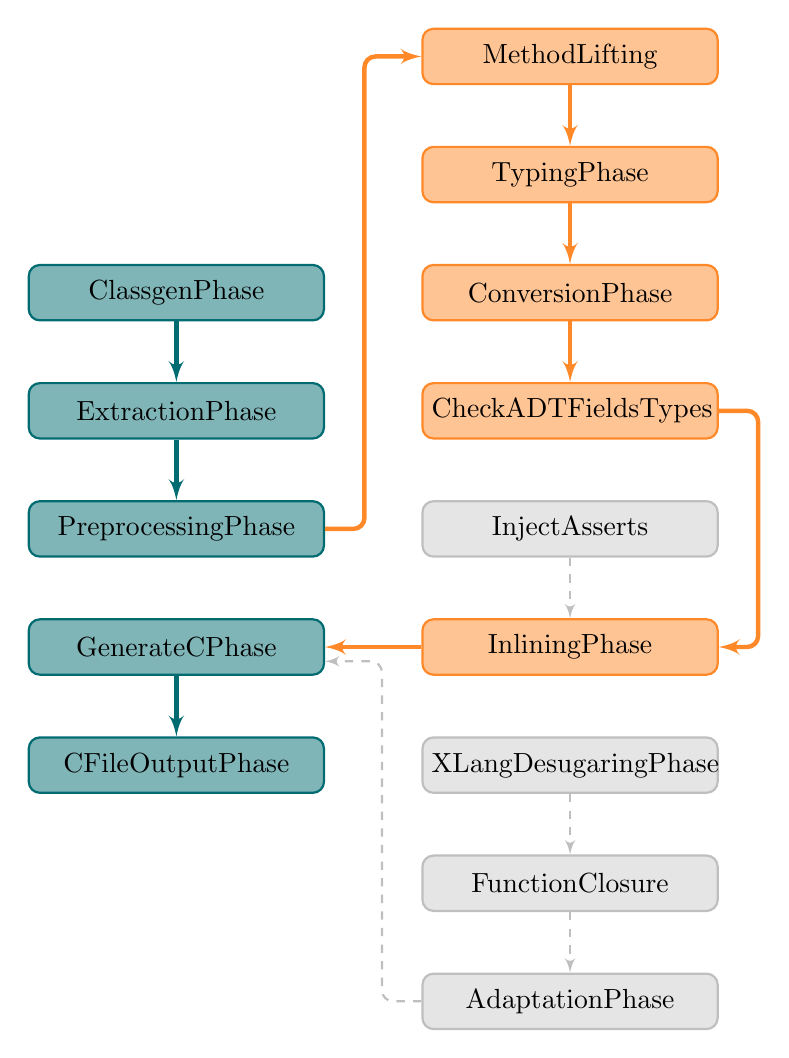
\begin{tikzpicture}[
      node distance=1.5cm,
      auto,
      box/.style={
        rectangle, draw=#1, thick, fill=#1!50,
        text width=10em, text centered, rounded corners,
        minimum height=2em
      },
      disabled box/.style ={
        rectangle, draw=gray!50, thick, fill=gray!20,
        text width=10em, text centered, rounded corners,
        minimum height=2em,
        %pattern=checkerboard light gray
      },
      line/.style={
        draw, -latex', ultra thick, rounded corners, c1
      },
      rectangle connector/.style={
        line,
        to path={(\tikztostart) -- ++(#1,0pt) \tikztonodes |- (\tikztotarget) },
        pos=0.5
      },
      disabled line/.style={
        line, gray!50, dashed, thick
      },
      disabled rectangle connector/.style={
        disabled line,
        to path={(\tikztostart) -- ++(#1,0pt) \tikztonodes |- (\tikztotarget) },
        pos=0.5
      },
    ]

    % column 2
    \node [box=c3] (d) {MethodLifting};
    \node [box=c3, below of=d] (e) {TypingPhase};
    \node [box=c3, below of=e] (f) {ConversionPhase};
    \node [box=c3, below of=f] (g) {CheckADTFieldsTypes};
    \node [disabled box, below of=g] (h) {InjectAsserts};
    \node [box=c3, below of=h] (i) {InliningPhase};
    \node [disabled box, below of=i] (j) {XLangDesugaringPhase};
    \node [disabled box, below of=j] (k) {FunctionClosure};
    \node [disabled box, below of=k] (l) {AdaptationPhase};

    % column 1
    \node [box=c1, left of=f, node distance=5cm] (a) {ClassgenPhase};
    \node [box=c1, below of=a] (b) {ExtractionPhase};
    \node [box=c1, below of=b] (c) {PreprocessingPhase};
    \node [box=c1, below of=c] (m) {GenerateCPhase};
    \node [box=c1, below of=m] (n) {CFileOutputPhase};

    % arrows
    \path [line] (a) -> (b);
    \path [line] (b) -> (c);
    \draw [rectangle connector=0.5cm, c3] (c.east) to (d);
    \path [line, c3] (d) -> (e);
    \path [line, c3] (e) -> (f);
    \path [line, c3] (f) -> (g);
    \path [rectangle connector=0.5cm, c3] (g.east) to (i.east);
    \path [disabled line] (h) -> (i);
    %\path [line, c3] ([yshift=1ex]i.west) -> ([yshift=1ex]m.east);
    \path [line, c3] (i.west) -> (m.east);
    \path [disabled line] (j) -> (k);
    \path [disabled line] (k) -> (l);
    \draw [disabled rectangle connector=-0.5cm] (l.west) to ([yshift=-1.2ex]m.east);
    \path [line] (m) -> (n);
  \end{tikzpicture}
  \endpgfgraphicnamed
  \caption{
    \GenC Pipeline when invoking Leon with \inlinecode{--genc}; \newline
    grey elements are disabled
  }
  \label{fig:genc-pipeline}
\end{figure}

The source code related to \GenC is stored in the
\inlinecode{src/main/scala/leon/genc/} direction of Leon's git repository. In
particular, the \inlinecode{CAST.scala} file contains a minimalistic AST for the
C language for the needs of this project, while \inlinecode{CConverter.scala}
holds most of the source code responsible for the conversion from the Scala AST
to the C one.



\section{Supported Features}

The current state of the \GenC phase supports programs using basic boolean and
integer types, tuples, arrays, non-recursive case classes, functions and nested
functions, \inlinecode{if} and \inlinecode{while} constructs and guarantees the
expressions execution order in the generated C99 program to be consistent with
the execution model of Scala.



\subsection{Types}
\label{sec:types}

In this section we give a summary of the different Scala types supported by
\GenC with their corresponding C99 types. We also detail the limitations on the
current state of Scala to safe C translation on the mentioned types.



\subsubsection{Basic Types}
\label{sec:basic-types}

Table~\ref{tab:basic-types} reports the three basis types that are currently
supported. In Scala, \inlineScala{Int} is subject to the same overflow behaviour
as the 32-bit integer type in C. Currently, Leon doesn't verify that no overflow
occurs but rather uses this behaviour to prove -- or disprove -- that some other
properties hold, such as the index used to read a value from an array is not
out-of-bound.

\begin{table}[h]
  \centering
  \begin{tabularx}{0.9\textwidth}{XX}
    \toprule

    \heading{Scala} & \heading{C99}               \\

    \midrule

    \inlineScala{Unit} & \inlineC{void}           \\

    \inlineScala{Boolean} &
    \inlineC{bool} (from \inlineC{<stdbool.h>})   \\

    \inlineScala{Int} (32-bit integer) &
    \inlineC{int32_t} (from \inlineC{<stdint.h>}) \\

    \bottomrule
  \end{tabularx}
  \caption{Supported basic types}
  \label{tab:basic-types}
\end{table}

The respective literals, such as \inlinecode{true}, \inlinecode{false}, and
numbers are supported as well, of course. Note that when extracting the Scala
AST, the compiler might convert some literals format, such as hexadecimal to
numbers in base 10. However, the Scala literal \inlineScala{(}) for the
\inlineScala{Unit} type has no equivalent in C99 and therefore is simply
ignored.



\subsubsection{Tuples}
\label{sec:tuples}

In addition to those basic types and their corresponding literals, \GenC also
supports generic tuples of size $N$. In Scala, tuples are represented with
different types according to their size: for example \inlineScala{(true, 1)} is
of type \inlineScala{Tuple2[Boolean, Int]} while \inlineScala{(2, false, 3)} is
of type \inlineScala{Tuple3[Int, Boolean, Int]}. In order to represent each
possible \inlineScala{TupleN[T1, ..., TN]} type in C99, without having access to
Scala's generics, we generate a new C structure for every combination of types
\inlineScala{T1, ..., TN} used in the original program, as a C++ templatised
structure would have generated at compilation time. The name of such structures
is defined by the concatenation of the combined types' name with
\inlineC{__leon_tuple} and \inlineC{_t} as prefix and postfix, respectively. The
field of those structures are simply matching the one from the source language.
Accessing elements of a tuple, say \inlineScala{_1}, is equivalently trivial in
C.

Listing~\ref{lst:example-tuple2} shows the equivalent C99 code that represents
\inlineScala{Tuple2[Boolean, Int]} type. In this particular case, having a
boolean field generates some padding in the memory layout of the structure.

%\begin{minipage}{\textwidth}
\pagebreak[3]
\begin{lstlisting}[
    language=C99,
    caption={Example of tuple type in C99},
    label={lst:example-tuple2},
    frame=trBL
  ]
typedef struct __leon_tuple_bool_int32_t_t {
  bool    const @_1@;  // padding
  int32_t const @_2@;
} __leon_tuple_bool_int32_t_t;
\end{lstlisting}
%\end{minipage}

Note that tuples can be made of other tuples, arrays or case classes at will.
However, the restrictions on arrays as discussed in
Section~\ref{sec:memory-limitations} also apply on tuples containing arrays.



\subsubsection{Case Classes}
\label{sec:case-classes}

\GenC also has a basic support for case classes. Currently it is restricted to
non-recursive types, without inheritance involved, where all member are values.
And, as with tuples, such data types can hold arrays as field with the
restriction mentioned in Section~\ref{sec:memory-limitations}. Essentially, case
classes are mapped to a C structure which fields are one-to-one C equivalent of
the Scala original type. Listing~\ref{lst:example-case-class} shows the C99
equivalent of declaring \inlineScala{case class Pixel(r: Int, g: Int, b: Int)}.

\begin{lstlisting}[
    language=C99,
    caption={Example of case class in C99},
    label={lst:example-case-class},
    frame=trBL
  ]
typedef struct Pixel0 {
  int32_t const @r0@;
  int32_t const @g0@;
  int32_t const @b0@;
} Pixel0;
\end{lstlisting}

Instantiating a case class is usually done using the compiler-defined companion
object of the same name. In C99, since there is no notion of constructor, we
have to rely on \emph{designated initialiser lists}.
Listing~\ref{lst:example-init-case-class} illustrates how \inlineScala{val red =
Pixel(255, 0, 0)} is converted into C99.

\begin{lstlisting}[
    language=C99,
    caption={Example of case class initialisation in C99},
    label={lst:example-init-case-class},
    frame=trBL
  ]
Pixel0 const red0 = (Pixel0) { @.r0@ = 255, @.g0@ = 0, @.b0@ = 0 };
\end{lstlisting}



\subsubsection{Arrays}
\label{sec:arrays}

Similarly to Scala's tuples, we handle the generic \inlineScala{Array[T]} type
by generating specific C99 structures for each \inlineScala{T} involved in the
source program. However, as the size of an array in Scala is not encoded into
its type, we cannot allocate a specific amount of memory with the matching C99
type definition. Instead, we create those structures with two fields: one
representing the length of the array and the other being a pointer to the memory
allocated for the array. We can delay the memory allocation to the instantiation
site of an array. The actual memory allocation is discussed in the next section.
Listing~\ref{lst:example-array} shows the corresponding type definition for a
\inlineScala{Array[(Boolean, Int)]} as an example.

\begin{lstlisting}[
    language=C99,
    caption={Example of tuple type in C99},
    label={lst:example-array},
    frame=trBL
  ]
typedef struct __leon_array___leon_tuple_bool_int32_t_t_t {
  __leon_tuple_bool_int32_t_t§*§ @data@;   // not owning the memory
  int32_t                      @length@;
} __leon_array___leon_tuple_bool_int32_t_t_t;
\end{lstlisting}

Independently on how an array is actually allocated, accessing one of its
elements is done through the usual C-array index access on its \inlineC{@data@}
field. Table~\ref{tab:example-array-access} shows a simple example of this.

\begin{table}[h]
  \centering
  \begin{tabular}{@{} c || l}
    \toprule

    \vheading{Scala} &
    \begin{lstlisting}[language=MyScala]
def foo(a: Array[Int]) = a(42)
    \end{lstlisting} \\

    \midrule

    \vheading{C99} &
    \begin{lstlisting}[language=C99]
int32_t foo0(__leon_array_int32_t_t const a0) {
  return a0.@data@§[§42§]§;
}
    \end{lstlisting} \\

    \bottomrule
  \end{tabular}
  \caption{Example of array access}
  \label{tab:example-array-access}
\end{table}



\subsubsection{Memory Model}
\label{sec:memory-limitations}

Since Scala's arrays have a fixed size once created, we don't have to implement
complex mechanism to properly resize arrays. Instead, we have to deal with two
main operations: allocating memory and deallocating it when appropriate. The
same is true for both tuples and case classes.

Because Leon currently doesn't allow aliasing on objects, the lifetime of
variables is trivial to deduce as only three scenarios can happen. First of all,
an objects can be a function parameter in which case the current function can
only observe its state without mutating it and no deallocation should happen
there as the current function doesn't own the memory. Secondly, it can be
created in a given function \inlineScala{f} and then returned. In this case, we
can consider the caller of \inlineScala{f} to own the memory and therefore it
falls in fact in the last case. Finally, a function can own an object if it
doesn't return it or have acquired it through one of its parameters. Hence, in
this case, the function is responsible to deallocate it when no longer needed.
This point in time is in the worst case when the function returns. It is
therefore safe to deallocate any owned piece of memory at this precise moment.

\begin{table}[b]
  \centering
  \begin{tabular}{@{} c || l}
    \toprule

    \vheading{Scala} &
    \begin{lstlisting}[language=MyScala]
val a = Array(1, 2, 3);
    \end{lstlisting} \\

    \midrule

    \vheading{C99} &
    \begin{lstlisting}[language=C99]
int32_t __leon_buffer0§[§3§]§ = { 1, 2, 3 };
__leon_array_int32_t_t const a3 = {
  @.length@ = 3,
  @.data@   = __leon_buffer0
};
    \end{lstlisting} \\

    \bottomrule
  \end{tabular}
  \caption{Example of fix-sized array}
  \label{tab:fix-sized-array}
\end{table}

The order in which the memory is deallocate needs not to be constrained by the
allocation order as no notion of destructor, as defined in C++ for example, is
present in Scala and therefore no ``late'' access to objects can happen.

Due to the restrictions imposed on some specific domains such as aircraft
software or some tiny embedded system regarding memory safety, we decided that,
in the first version of \GenC, no manual allocation should be done and instead
only stack-allocated objects can be created. This is of course a very
restrictive decision as it implies returning arrays is not possible without
moving the allocation site to the caller when the array is returned from a
function. In fact, if the size of a returned array is not known at compile time
it becomes even more arduous to handle. A solution to this specific problem
could be to inline the called function directly in the generated C code.

However, in order to have a working implementation decently quickly we decided
to forbid returning arrays and types containing arrays. This restriction doesn't
apply to other tuples or case classes thanks to the no-aliasing policy of Leon
which implies that copying a returned variable of fixed size is valid. Note that,
due to the fact that the length of arrays is not encoded in the type, we cannot
relax this restriction to arrays of fixed length as this information is not
available to the caller.

\begin{table}[t]
  \centerfloat
  \begin{tabular}{@{} c || l}
    \toprule

    \vheading{Scala} &
    \begin{lstlisting}[language=MyScala]
def foo(size: Int, value: Int) {
  val a = Array.fill(size)(value)
}
    \end{lstlisting} \\

    \midrule

    \vheading{C99} &
    \begin{lstlisting}[language=C99]
void foo0(int32_t const size0, int32_t const value0) {
  int32_t __leon_vla_buffer0§[§size0§]§;
  for (int32_t __leon_i1 = 0; __leon_i1 < size0; ++__leon_i1) {
    __leon_vla_buffer0§[§__leon_i1§]§ = value0;
  }
  __leon_array_int32_t_t const a3 = {
    @.length@ = size0,
    @.data@   = __leon_vla_buffer0
  };
}
    \end{lstlisting} \\

    \bottomrule
  \end{tabular}
  \caption{Example of runtime allocated array}
  \label{tab:vla}
\end{table}

With that in mind, we can deal with array allocation in two ways. First, for
fix-sized array we can use regular C-array as shown in
Table~\ref{tab:fix-sized-array}: a buffer of the corresponding size is allocated
on the stack and then an instance of the corresponding array type is created
with the \inlineC{@data@} field pointing to the allocated buffer and the
\inlineC{@length@} field being initialised appropriately. This buffer will get
automatically deallocated when the program reaches the end of its scope. When
the size of the array is only known at runtime we can rely on Variable Length
Array (VLA) to create the memory buffer representing the array as shown in
Table~\ref{tab:vla}: instead of being statically defined, the size of the buffer
is determined dynamically but the its lifetime remains the same.



\subsection{Variables}

Among the many differences between Scala and C is the immutability idiom used in
functional languages compared to the constness expressed in imperative
languages. For a basic type \inlineScala{T}, such as \inlineScala{Int} or
\inlineScala{Boolean}, having in Scala \inlineScala{val x: T = ...} corresponds
to having \inlineC{T const x = ...} in C.

Regarding arrays, even if they are declared as \inlineScala{val}, the elements
of the arrays can still be mutated\footnote{Leon currently restricts, due to
aliasing issues, the update of arrays to the ones declared locally. Hence,
passing an array as parameter make it read only.}. This is reflected in C as
well by using a pointer to represent the beginning of the memory allocated for
the array: whether or not an instance of \inlineC{__leon_array_T_t} is marked
with \inlineC{const}, the \inlineC{@data@} field gives read and write access to
the elements of the array.

As for compound data types such as tuples or case classes, we can simply mark as
\inlineC{const} any instance of those types as \GenC currently support only
immutable case classes and because tuples are defined to be immutable in Scala.



\subsection{Functions}

The support for functions in \GenC is relatively complete from an imperative
point of view. That is, first-order functions are supported as well as nested
functions but higher-order functions are not. Additionally, since strings of
characters are not yet implemented, the main function should be defined in Scala
as \inlineScala{def main: Int = ...}.

During the extraction of the Scala AST, the variable, function and class
identifiers are renamed as to avoid any ambiguity. This is why two functions
originally named \inlineScala{foo} in the input source code, were they declared
in different scopes or simply overloads, would be renamed into
\inlineScala{foo0} and \inlineScala{foo1} in the AST. The direct consequence of
this is that function overloading is directly supported by \GenC without extra
work.



\subsubsection{Nested Functions}

In order to support nested functions, which don't exist in vanilla C, we have to
outline nested functions without modifying the scope of variables. The idea is
to add extra parameters to extracted functions to extend the function's context
to include what was available in the original source code.

However, in C parameters are pass-by-value and therefore copied while in Scala
arguments are either pass-by-name, which \GenC does not support at the moment,
or pass-by-reference (to use in C-terminology). This in itself means that if a
nested function mutates a variable created in the outer function, the effect
using pass-by-value in C to share the variable would not allow the extracted
function to have the desired side-effect. We therefore have to use pointer to
simulate the pass-by-reference nature of Scala parameters when calling a nested
function and dereference pointers when accessing those variables.

Table~\ref{tab:example-nested1} illustrates how we can handle 1-level nested
function. For deeper nested functions we have an additional issue: parameters
that were already pointers-to-value should not be transformed into pointer to
pointers. Table~\ref{tab:example-nested2} shows an example that correctly handle
this case.

\begin{table}[h]
  \centerfloat
  \begin{tabular}{@{} c || l}
    \toprule

    \vheading{Scala} &
    \begin{lstlisting}[language=MyScala]
def foo(x: Int) = {
  def bar(y: Int) = x * y
  bar(2)
}
    \end{lstlisting} \\

    \midrule

    \vheading{C99} &
    \begin{lstlisting}[language=C99]
int32_t bar0(int32_t const@*@ x0, int32_t const y6) {
  return (£(*x0)£ * y6);
}

int32_t foo0(int32_t const x0) {
  return bar0(@(&x0)@, 2);
}
    \end{lstlisting} \\

    \bottomrule
  \end{tabular}
  \caption{Example of simply nested functions}
  \label{tab:example-nested1}
\end{table}

\begin{table}[h]
  \centerfloat
  \begin{tabular}{@{} c || l}
    \toprule

    \vheading{Scala} &
    \begin{lstlisting}[language=MyScala]
def foo(x: Int) = {
  def bar(y: Int) = {
    def fun(z: Int) = x * y + z
    fun(3)
  }
  bar(2)
}
    \end{lstlisting} \\

    \midrule

    \vheading{C99} &
    \begin{lstlisting}[language=C99]
int32_t fun0(int32_t const@*@ x0, int32_t const@*@ y6, int32_t const z9) {
  return ((£(*x0)£ * £(*y6)£) + z9);
}

int32_t bar0(int32_t const@*@ x0, int32_t const y6) {
  return fun0(§x0§, @(&y6)@, 3);
}

int32_t foo0(int32_t const x0) {
  return bar0(@(&x0)@, 2);
}
    \end{lstlisting} \\

    \bottomrule
  \end{tabular}
  \caption{Example of deeply nested functions}
  \label{tab:example-nested2}
\end{table}



\subsection{Statements}

\GenC provides support for converting basic operators, \inlinecode{if}- and
\inlinecode{while}-constructs to C99 as described next by ensuring a consistent
execution of instructions as well as converting traditional functional form to
imperative style.



\subsubsection{Operators}

The support for operators is shown in Table~\ref{tab:operators}. Note that both
unary and binary minus operators are supported -- but Scala's \inlineScala{>>>}
is not -- and that the effect of operators is the same in both languages.
Additionally, the precedence of operators, even though roughly equivalent, is
guaranteed in the generated code by wrapping every sub-expressions in
parentheses conformally to Scala operator priority hierarchy.

\begin{table}[h]
  \centering
  \begin{tabular}{lc}
    \toprule
    \heading{Category}                 & \heading{Operators}         \\
    \midrule
    Boolean operators                  & \inlineC{\&\& \|\| ! != ==} \\
    Comparison operators over integers & \inlineC{< <= == != >= >}   \\
    Arithmetic operators over integers & \inlineC{+ - * / \%}        \\
    Bitwise operators over integers    & \inlineC{\& \| ^ - << >>}   \\
    \bottomrule
  \end{tabular}
  \caption{Supported operators}
  \label{tab:operators}
\end{table}



\subsubsection{\inlinecode{if}-Construct}

One major difference between conditional branching in Scala vs C is the ability
to assign a variable to the value generated by an \inlineScala{if}-construct in
Scala. \GenC handles these situations by transforming values into variables and
assigns the appropriate value inside the \textit{then} or \textit{else} branches
of the \inlineC{if}-statement in C. Similarly, when an
\inlineScala{if}-construct is used as the last instruction of a function, Scala
will return it. In C99, instead of creating a temporary variable and then
returning it, \GenC injects a \inlineC{return} statement in both branches of the
conditional branching. Table~\ref{tab:example-if} shows examples of this kind of
conversions.

\begin{table}[t]
  \centering
  \begin{tabular}{@{} c || l}
    \toprule

    \vheading{Scala} &
    \begin{lstlisting}[language=MyScala]
def abs(x: Int) = if (x >= 0) x else -x

def fun(b: Boolean) {
  val x = if (b) 42 else 58
  // ...
}
    \end{lstlisting} \\

    \midrule

    \vheading{C99} &
    \begin{lstlisting}[language=C99]
int32_t abs0(int32_t const x0) {
  if ((x0 >= 0)) { return x0; }
  else { return (-x0); }
}

void fun0(bool const b0) {
  int32_t x8; // no const here
  if (b0) { x8 = 42; }
  else { x8 = 58; }
  // ...
}
    \end{lstlisting} \\

    \bottomrule
  \end{tabular}
  \caption{Examples of \inlinecode{if}-construct conversions}
  \label{tab:example-if}
\end{table}



\subsubsection{\inlinecode{while}-Construct}

Basic \inlineScala{while}-construct are supported rather straightforwardly by
\GenC as the meaning of this keyword is the same in both languages.
Table~\ref{tab:example-simple-while} illustrates this. However, when nested
instructions are put inside the loop condition, the conversion becomes slightly
more tricky as exposed in Section~\ref{sec:normalisation}.

\begin{table}[h]
  \centering
  \begin{tabular}{@{} c || l}
    \toprule

    \vheading{Scala} &
    \begin{lstlisting}[language=MyScala]
def sum(a: Array[Int]): Int = {
  var i = 0
  var acc = 0
  while (i < a.length) {
    acc = acc + a(i)
    i = i + 1
  }
  acc
}
    \end{lstlisting} \\

    \midrule

    \vheading{C99} &
    \begin{lstlisting}[language=C99]
int32_t sum0(__leon_array_int32_t_t const a0) {
  int32_t i9 = 0;
  int32_t acc1 = 0;
  while ((i9 < a0.length)) {
    acc1 = (acc1 + a0.data[i9]);
    i9 = (i9 + 1);
  }
  return acc1;
}
    \end{lstlisting} \\

    \bottomrule
  \end{tabular}
  \caption{Example of \inlinecode{while}-construct conversions}
  \label{tab:example-simple-while}
\end{table}



\subsubsection{Execution Order Normalisation}
\label{sec:normalisation}


On the one hand, we have Scala, based on JVM runtime, that enforces a strict
order of instruction execution at runtime. Generally speaking, Scala executes
statement from left to right. On the other hand, we have the C standard that
specifies a rather flexible order of execution. Compiler manufacturers can
choose to re-order instructions in order to optimise code. The C99 standard
defines the behaviour of program execution through Sequence
Points\footnote{Refers to Section 5.1.2.3 and Annex C of the C99 standard for
the complete definition of sequence points.} and Undefined Behaviour. As a
direct consequence, expressions are often not executed from left to right but in
a implementation-specific order. Depending on the compiler and target
architecture, the same C code can present different behaviours. We therefore
have to be careful when converting instructions from Scala to C in order to
prevent operations with side-effect to work differently in both languages but
also with all C compilers and target architectures.

There are specific areas of code where this issue is fundamentally important.
For example in Table~\ref{tab:example-exec-order-function}, when invoking the
function \inlineScala{foo} with its two arguments, both parameters need to be
evaluated from left to right. \GenC makes sure that the sequence points match
the behaviour of the original program by creating intermediary variables
wherever needed.

\begin{table}[h]
  \centerfloat
  \begin{tabular}{@{} c || l}
    \toprule

    \vheading{Scala} &
    \begin{lstlisting}[language=MyScala]
def example = {
  var counter = 0;
  def get() = {
    counter = counter + 1
    counter
  }
  def foo(x: Int, y: Int) = {
    if (x < y) true
    else       false
  }

  foo(get(), get())
}
    \end{lstlisting} \\

    \midrule

    \vheading{C99} &
    \begin{lstlisting}[language=C99]
int32_t get2(int32_t* counter0) {
  (*counter0) = ((*counter0) + 1);
  return (*counter0);
}

bool foo0(int32_t* counter0, int32_t const x7, int32_t const y6) {
  if ((x7 < y6)) { return true; }
  else { return false; }
}

bool example0(void) {
  int32_t counter0 = 0;
  int32_t const __leon_normexec0 = get2((&counter0));
  int32_t const __leon_normexec1 = get2((&counter0));
  return foo0((&counter0), __leon_normexec0, __leon_normexec1);
}
    \end{lstlisting} \\

    \bottomrule
  \end{tabular}
  \caption{Example of execution normalisation of function call in C99}
  \label{tab:example-exec-order-function}
\end{table}

In addition to the execution normalisation of function parameters, \GenC
extracts nested statements in operands and branching conditions, while
preserving short-circuiting in boolean operations but regardless of operator
precedence.  Tables \ref{tab:example-exec-order-operands} and
\ref{tab:example-exec-order-short-circuiting} illustrate those two scenarios. In
the first example, sub-expressions can simply be lifted outside their respective
block by transforming the left-to-right ordering into top-to-bottom. In the
second example, boolean conjunction and disjunction operators are replaced by
their equivalent \inlineC{if}-statement. Additionally, the unnecessary last term
was removed from the C translation, thanks to the short circuiting rules.

A slightly more complex normalisation example is shown in
Table~\ref{tab:example-exec-order-while} where a \inlineScala{while}-statement
needs to be expressed in terms of an infinite loop with a break condition in
order to accommodate for the boolean condition having some side-effect and
therefore requiring to be re-evaluated at each loop iteration. Furthermore,
since the second conditional operand has no side-effect, the resulting decision
tree is compressed into two \inlineC{if}-statements instead of three.

\begin{table}[h]
  \centerfloat
  \begin{tabular}{@{} c || l}
    \toprule

    \vheading{Scala} &
    \begin{lstlisting}[language=MyScala]
def example(j: Int) = {
  var c = 0
  val x = { c = c + 3; j } +
          { c = c + 1; j } * { c = c * 2; j }
  c == 8
}
    \end{lstlisting} \\

    \midrule

    \vheading{C99} &
    \begin{lstlisting}[language=C99]
bool example0(int32_t const j0) {
  int32_t c2 = 0;
  c2 = (c2 + 3);
  c2 = (c2 + 1);
  c2 = (c2 * 2);
  int32_t const x7 = (j0 + (j0 * j0));
  return (c2 == 8);
}
    \end{lstlisting} \\

    \bottomrule
  \end{tabular}
  \caption{Example of execution normalisation for operands in C99}
  \label{tab:example-exec-order-operands}
\end{table}

\begin{table}[h]
  \centerfloat
  \begin{tabular}{@{} c || l}
    \toprule

    \vheading{Scala} &
    \begin{lstlisting}[language=MyScala]
def example(b: Boolean) = {
  val f = b && !b // == false
  var c = 0
  val x = f || { c = 1; true } || { c = 2; false }
  c == 1
}
    \end{lstlisting} \\

    \midrule

    \vheading{C99} &
    \begin{lstlisting}[language=C99]
bool example0(bool const b0) {
  bool const f26 = (b0 && (!b0));
  int32_t c2 = 0;
  bool x7;
  if (f26) { x7 = true; }
  else {
    c2 = 1;
    x7 = true;
  }
  return (c2 == 1);
}
    \end{lstlisting} \\

    \bottomrule
  \end{tabular}
  \caption{Example of execution normalisation with short-circuiting in C99}
  \label{tab:example-exec-order-short-circuiting}
\end{table}

\begin{table}[h]
  \centerfloat
  \begin{tabular}{@{} c || l}
    \toprule

    \vheading{Scala} &
    \begin{lstlisting}[language=MyScala]
def example(b: Boolean) = {
  var i = 10
  var c = 0

  val f = b && !b // == false
  val t = b || !b // == true

  // The following condition is executed 11 times,
  // and only during the last execution is the last
  // operand evaluated
  while ({ c = c + 1; t } && i > 0 || { c = c * 2; f }) {
    i = i - 1
  }

  i == 0 && c == 22
}
    \end{lstlisting} \\

    \midrule

    \vheading{C99} &
    \begin{lstlisting}[language=C99]
bool example0(bool const b0) {
  int32_t i9 = 10;
  int32_t c2 = 0;
  bool const f26 = (b0 && (!b0));
  bool const t8 = (b0 || (!b0));

  while (true) {
    c2 = (c2 + 1);
    if ((t8 && (i9 > 0))) { /* empty */ }
    else {
      c2 = (c2 * 2);
      if (f26) { /* empty */ }
      else { break; }
    }

    i9 = (i9 - 1);
  }

  return ((i9 == 0) && (c2 == 22));
}
    \end{lstlisting} \\

    \bottomrule
  \end{tabular}
  \caption{Example of execution normalisation of \inlinecode{while}-statement in C99}
  \label{tab:example-exec-order-while}
\end{table}



\FloatBarrier
\subsubsection{Ignored Features}

The following Scala statements are ignored by \GenC as they should have no
side-effect except decreasing the runtime performance: \inlineScala{require}
(pre-conditions), \inlineScala{ensuring} (post-conditions) and
\inlineScala{assert}. It is expected from the user that those statements were
verified using Leon verification mechanisms.



\section{Case Study}
\label{sec:case-study}

To assess the quality of this project, a case study showcasing basic image
processing was implemented in Scala and verified using Leon and then converted
to C99 using its \GenC phase. Appendices \ref{sec:case-study-input-code} and
\ref{sec:case-study-output-code} report the Scala source code and its analogous
C99 code. This example highlights the current capability of Leon to generate
safe C code, but also shows where it should be improved.

The code can be verified using: \newline \centerline{ \inlinecode{leon --xlang
--solvers=smt-z3,ground IntegralColor.scala} } \newline and converted to C99
with: \newline \centerline{\inlinecode{leon --xlang --genc --o=IntegralColor.c
IntegralColor.scala}}

The first limitation is the absence of support for floating point types such as
\inlineC{double} in C. This limitation is due to the complexity involved when
proving properties about such variables. Therefore, one has to convert
operations on real numbers into integer operations, which can substantially
complexify algorithms such as in image processing algorithms.

A second serious limitation is the impossibility to mutate array passed as
parameter to functions or to return arrays from functions. This is,
respectively, due to aliasing of variables, which makes it harder to prove some
properties, and to the simple memory model currently implemented by \GenC.
Hence, the modularity of the code is significantly impacted: for example, it is
not possible to define a function that converts an arbitrary RGB-image into
greyscale using arrays. Instead, one has to duplicate code in order to apply,
say smoothing, to any image.

However, we were able to prove the correctness of this case study -- which
exhibits close to every supported concepts -- and the produced C99 code could be
successfully compiled using Clang. Furthermore, when executed, the generated
program shows the appropriate behaviour.



\section{Future Development}

In this initial version of \GenC, we were able to support not only basic types
such as boolean or 32-bit integer, but also generate appropriate code to define
and use tuple of arbitrary types, immutable case classes and stack-allocated
arrays of either fixed size or runtime size. The distinction between
\inlineScala{val} and \inlineScala{var} for those types and the idiom of
mutability were applied to C program through constness. Additionally, overloads
of functions and nested functions were properly converted to the namespace-less
C language. Finally, imperative code instructions such as \inlinecode{if}- or
\inlinecode{while}-statements, as well as usual operators on the supported basic
types, were translated appropriately, enforcing a consistent execution order of
expressions for both languages.

The next steps of development for this module of Leon are multiple. On a general
level, Leon and \GenC could be extended to support verifying some properties
about floating point types, or to ensure that no overflow occurs, but also by
supporting additional integral types such as 16-bit or 64-bit integers.

\GenC could also be improved by providing a more complex memory model that
supports heap-allocation. Since this feature might not be usable on some
devices, it would probably be safer to make it opt-in through a command line
flag. This advanced model would help writing modular code such as discussed in
Section~\ref{sec:case-study}.

An important part of code written in Scala is based on functional features. One
of the major features being higher-order functions, supporting them in \GenC
would significantly improve the range of program that could be safely converted
to C99.

Regarding functions, currently \GenC considers every function to have
side-effect. Execution normalisation as presented in
Section~\ref{sec:normalisation} could benefit from detecting which function can
have side-effect for the current statement to generate code that not only would
be easier to read but also let C compilers perform optimisations at will.
Moreover, while not always necessarily useful in practice since C compiler are
allowed to remove unused parameters to optimise code, the parameters of
extracted nested functions could be reduced to the minimal set of variables that
are accessed.

Finally, some secondary details could be improved such as the pretty printer to
improve code readability: extra parentheses could be removed and identifiers
could be kept as they are in the input source code where there is no ambiguity
due to name clashing in a namespace-less language such as C. We however believe
that improving further the pretty printer regarding the formatting of the
produced code would not be useful since some advanced tools are already
independently developed and widely used.



\appendix



\clearpage
\section{Case Study: IntegralColor.scala}
\label{sec:case-study-input-code}

\lstinputlisting[language=MyScala, style=LongCode]{IntegralColor.scala}



\clearpage
\section{Case Study: Generated IntegralColor.c}
\label{sec:case-study-output-code}

\lstinputlisting[language=C99, style=LongCode]{IntegralColor.c}



\end{document}

% vim: spell spelllang=en_gb
% vim: set tabstop=2 softtabstop=2 shiftwidth=2 textwidth=80: %

